%%%% Weekly Report Information %%%%
\newcommand{\handoutName}{Weekly report}
\newcommand{\handoutdate}{Nov 25, 2014}
\newcommand{\duedate}{}
% Header template used for Weekly Reports
\documentclass[11pt,twoside]{article}

\setlength{\oddsidemargin}{0pt}
\setlength{\evensidemargin}{0pt}
\setlength{\textwidth}{6.5in}
\setlength{\topmargin}{0in}
\setlength{\textheight}{8.5in}
\setlength{\voffset}{0in}

\providecommand{\titlesize}{small}


\usepackage{graphicx}
%\usepackage{subfigure}
\usepackage{palatino}
%\usepackage{cmbright}
\newcommand{\myMargin}{1.00in}
%\usepackage[pdftex]{hyperref}
\usepackage[small,bf]{caption}
\usepackage{amsmath}
\usepackage[usenames,dvipsnames]{color}
\usepackage{fancyhdr}
\pagestyle{fancy}
\usepackage{datetime}
\usepackage{fancyvrb}
\usepackage{color}
\usepackage[\titlesize, compact]{titlesec}
\usepackage{multicol}
\usepackage{enumitem}
\usepackage{pdfpages}
\usepackage{mdwlist}


\usepackage[ruled]{algorithm}
\usepackage{algpseudocode}

\usepackage{caption}
\usepackage{subcaption}



\newdateformat{dashdate}{\THEYEAR-\twodigit{\THEMONTH}-\twodigit{\THEDAY}}
\def\Tiny{\fontsize{3pt}{3pt}\selectfont}

\providecommand{\handoutName}{Handout title}
\providecommand{\handoutdate}{Handout date}
\providecommand{\duedate}{}

\lhead{Meeting with Prof. Becker\\
Fall, 2014}
\chead{}
\rhead{ Shiva Shahrokhi\\
\handoutdate }
\lfoot{}
\cfoot{\thepage}
\rfoot{\dashdate \Tiny \textcolor{Gray}{\today}}
\renewcommand{\headrulewidth}{0.4pt}
\renewcommand{\footrulewidth}{0.4pt}

\begin{document}

\vspace{0.60in}
\begin{center}
{\Large\textbf{\handoutName}}\\
\vspace{0.03in}
\textbf{\duedate}\\
\end{center}

\newcommand{\todo}[1]{
  \textcolor{Red}{
    \begin{tabular}{|c|}
      \hline
      \em \large \bfseries todo: \normalfont \normalsize #1 \\
      \hline
    \end{tabular}}
}


\section{My \emph{Objectives} this week}
\begin{itemize}
\item Adding a S shape and obstacle, Grid view of the surface.
\item implement brushfire Algorithm
\item shape the paper in new format
\end{itemize}


\section{My \emph{Accomplishments} this week}

\subsection{\emph{Auto Control}}

\begin{itemize}
\item Grid View
\end{itemize}




\begin{figure}
        \centering
         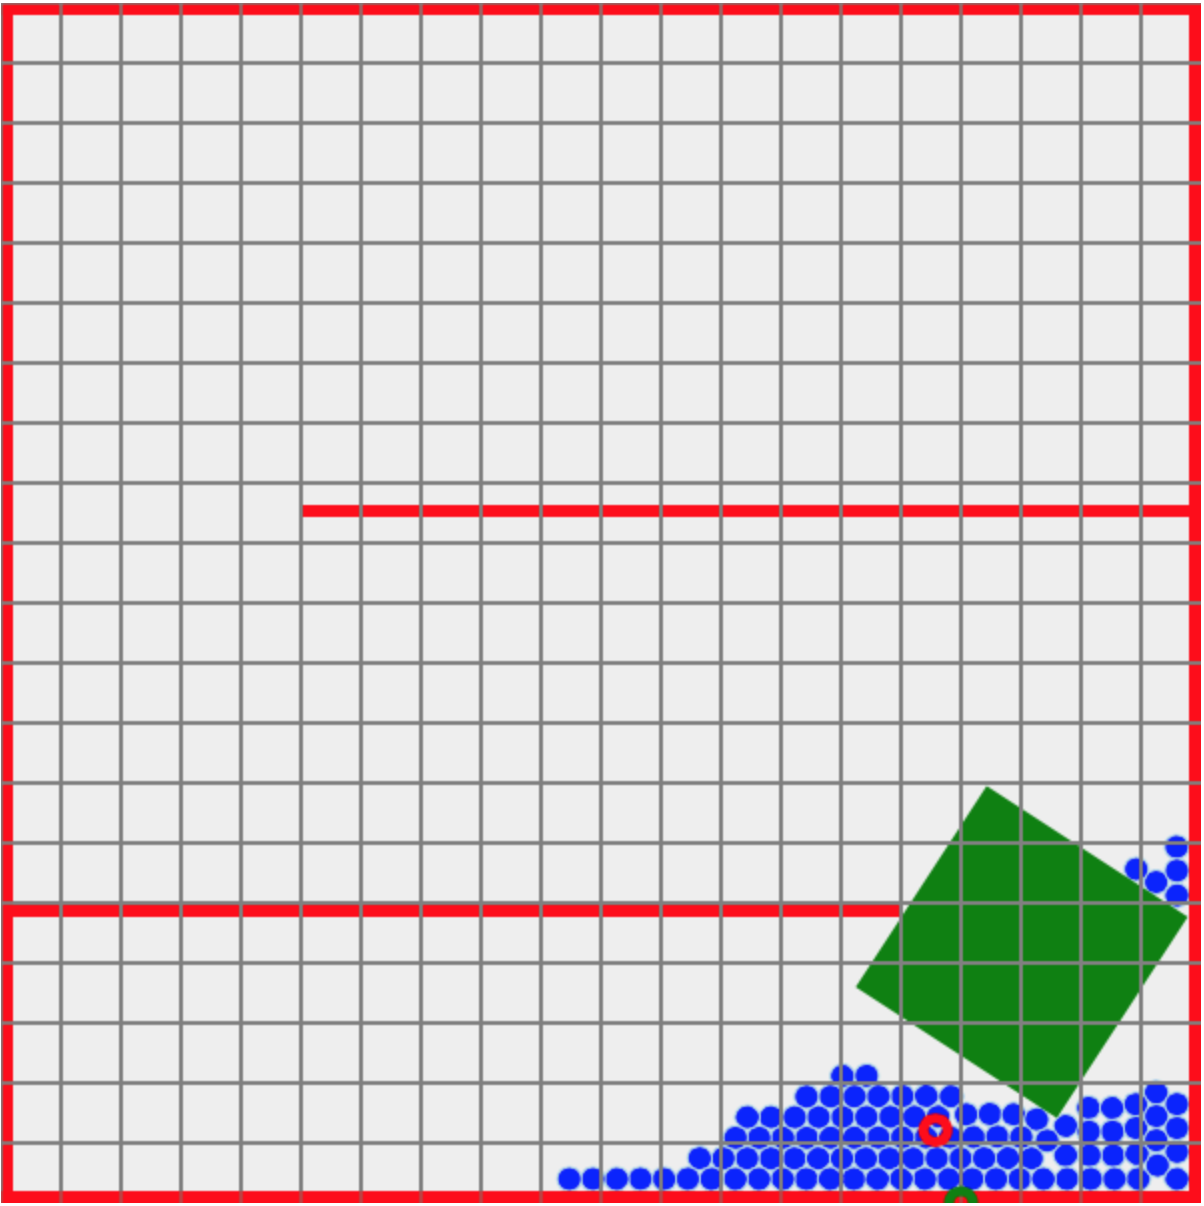
\includegraphics[width=0.3\textwidth]{fig/GridView.png}
                \caption{Grid View }
                \label{fig:gull}
        
\end{figure}


\begin{itemize}
\item Implementing Brushfire Algorithm
\end{itemize}

My problem with brushfire algorithm is that I didn't understand how it works completely. I modified it a little bit by this algorithm:
\begin{itemize}
\item I first of all, give a default value of infinity to obstacles, and give zero to all the spaces. I give one to the goal, and run the algorithm.
\item every node neighboring goal with get value of the goal + 1
\item every node neighboring their neighbors get the least value of their neighbors +1
\item I don't count 0 as a number.
\end{itemize}
I run this algorithm until it reaches the start position.
But it has some difficulties, because we can not reach the goal always, because of the standard deviation. we should expect that we have reached the goal, if we are as near as doubled standard deviation to it.

\begin{itemize}
\item Reshaping Paper
\end{itemize}




\section{My \emph{Plan} for next week}

\begin{itemize}
\item Complete the algorithm: 1. Going to static obstacles if the variance was less than something, and going behind the object to push it otherwise. 
\item write the Lyapunov's proof for the controlling variance.
\end{itemize}

\subsection{Meeting with Dr. Becker On Tuesday, 12 pm }

\begin{itemize}
\item To see if my algorithm work

\item Show him results.
\end{itemize}

\end{document}
